\section{Verification and comparison with NHWAVE and REEF3D::NHFLOW}
\label{sec:verification}

This section collects the first round of tests. Where possible, the
benchmarks were also run with two established non-hydrostatic $\sigma$-layer
models on the same set-up: the same domain, bottom, gauges, horizontal spacing
and number of layers. Each model keeps its own numerics and its usual wave
input (Table~\ref{tab:models}). Unless stated otherwise, \NHFOAM\ uses the
interface pressure, \code{limitedLinearV}, BDF2 and one outer corrector without
flux extrapolation, i.e.\ the settings before the fixes of
Section~\ref{sec:ma2012}.

\begin{table}[ht]
\centering
\caption{The three models compared in Sections~\ref{sec:verification} and
\ref{sec:ma2012}.}
\label{tab:models}
\small
\begin{tabular}{p{3.0cm}p{3.6cm}p{3.6cm}p{3.6cm}}
\toprule
 & \NHFOAM & NHWAVE & REEF3D::NHFLOW \\
\midrule
version & this repository & \code{JimKirby/NHWAVE} master (1483007), MPI and HYPRE 3.2 & 26.08 (conda-forge build) \\
vertical pressure & layer interfaces (default) or cell centres & layer interfaces & as distributed \\
advection, time & see text; BDF2 & HLPA (TVD), second-order Runge--Kutta & WENO, HLL fluxes \\
time step (bar) & fixed, 5 ms & adaptive, CFL 0.5 ($\approx$4.6 ms) & adaptive, CFL 1 ($\approx$9.7 ms) \\
wave input (bar) & 8 m relaxation zone, linear & linear, at the left boundary & 8 m relaxation zone, linear \\
absorption (bar) & 8 m sponge & 8 m sponge & 8 m relaxation zone \\
\bottomrule
\end{tabular}
\end{table}

\subsection{Basic checks}
\label{sec:basic}

Table~\ref{tab:basic} lists the basic checks; Figs.~\ref{fig:basin3d} and
\ref{fig:solitary01} show two of them.

\begin{table}[ht]
\centering
\caption{Basic checks (interface pressure unless noted).}
\label{tab:basic}
\small
\begin{tabular}{p{6.3cm}p{8.7cm}}
\toprule
test & result \\
\midrule
still water over the bar bathymetry (1:20 and 1:10 slopes), 10 s & $\eta\equiv 0$ (exact); $\max|\bm{u}| < 10^{-12}$ m/s, exactly 0 at the end \\
volume conservation, closed basins & round-off: $10^{-14}$ m$^3$ or less (2DV and 3D) \\
standing wave, $kh=1$, 10 layers, $T/\Delta t = 200$ & period $+0.04\%$, amplitude $-0.04\%$ over $4.5\,T$ (cell layout $+0.13\%$, $-0.03\%$) \\
solitary wave, $H/h = 0.1$, 10 layers & speed 3.283 m/s between $x=10$ and 30 m, against $\sqrt{g(h+H)} = 3.285$ m/s; height $-0.2\%$ from $x=10$ to 40 m \\
circular basin, 3D unstructured prisms, 8 layers & period $+0.07\%$ against the analytical Bessel mode (cell layout $+0.20\%$) \\
serial vs 2 processors (solitary wave crossing the processor boundary) & $\max|\Delta\eta| = 7\times10^{-8}$ m for $H = 0.1$ m \\
bottom uplift, $\zeta_0/h = 0.01$, 5 layers & peaks within 1.5\% of linear potential theory up to $x/b = 20$; volume conserved to $10^{-16}$ m$^3$ \\
\bottomrule
\end{tabular}
\end{table}

\begin{figure}[ht]
\centering
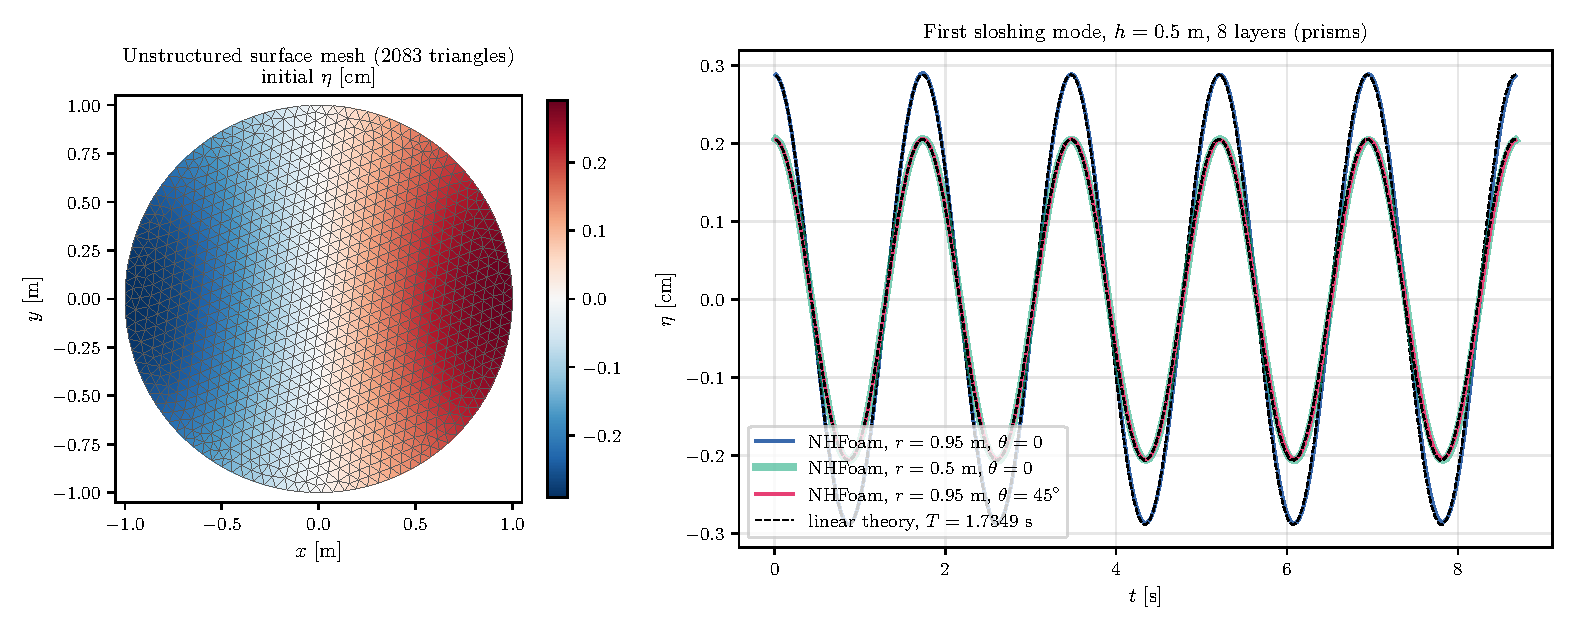
\includegraphics[width=\textwidth]{circular_basin_3d.pdf}
\caption{First sloshing mode of a circular basin ($R=1$ m, $h=0.5$ m) on an
unstructured mesh of triangular prisms, 8 layers: surface mesh with the
initial elevation, and gauges against linear theory.}
\label{fig:basin3d}
\end{figure}

\begin{figure}[ht]
\centering
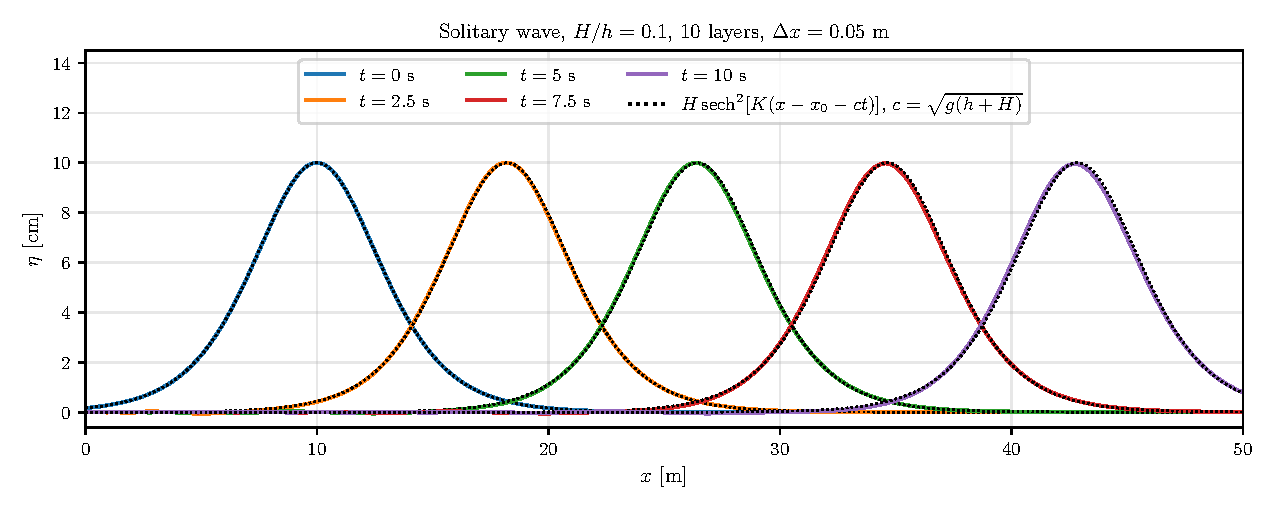
\includegraphics[width=\textwidth]{solitary_wave.pdf}
\caption{Solitary wave of $H/h=0.1$, 10 layers, $\Delta x = 0.05$ m: profiles
against the initial $\mathrm{sech}^2$ shape moved at $c=\sqrt{g(h+H)}$.}
\label{fig:solitary01}
\end{figure}

\FloatBarrier
\subsection{Dispersion and the number of layers}
\label{sec:dispersion}

Standing waves in closed basins, with 64 cells per wavelength,
$T/\Delta t = 200$ and uniform layers, give the period error of
Table~\ref{tab:dispersion} and Fig.~\ref{fig:dispersion}, measured over 4.5
periods. With the pressure on the interfaces, two layers keep the period error
within 0.6\% up to $kh=7$ and three layers within 0.21\%. With five or more
layers, what is left ($-0.04$ to $+0.07\%$) comes from $\Delta x$ and $\Delta t$.
The cell-centred layout needs about 3 layers for $kh\le1$, 5--6 for $kh\le2$,
10 for $kh\le4$ and 20 for $kh\le7$ to stay within 1\%.

\begin{table}[ht]
\centering
\caption{Period error of standing waves [\%] for $kh = 1$ / 3 / 7.}
\label{tab:dispersion}
\small
\begin{tabular}{rll}
\toprule
layers & interface layout (default) & cell layout \\
\midrule
1  & $-2.4$ / $+3.9$ / $+38$       & $+6.9$ / $+35$ / $+91$ \\
2  & $-0.52$ / $-0.16$ / $+0.61$   & $+1.9$ / $+12$ / $+42$ \\
3  & $-0.20$ / $-0.06$ / $+0.05$   & $+0.88$ / $+5.9$ / $+24$ \\
5  & $-0.03$ / $+0.01$ / $+0.05$   & $+0.36$ / $+2.2$ / $+10.5$ \\
10 & $+0.04$ / $+0.04$ / $+0.05$   & $+0.13$ / $+0.61$ / $+3.0$ \\
20 & $+0.06$ / $+0.05$ / $+0.04$   & $+0.08$ / $+0.19$ / $+0.79$ \\
\bottomrule
\end{tabular}
\end{table}

\begin{figure}[ht]
\centering
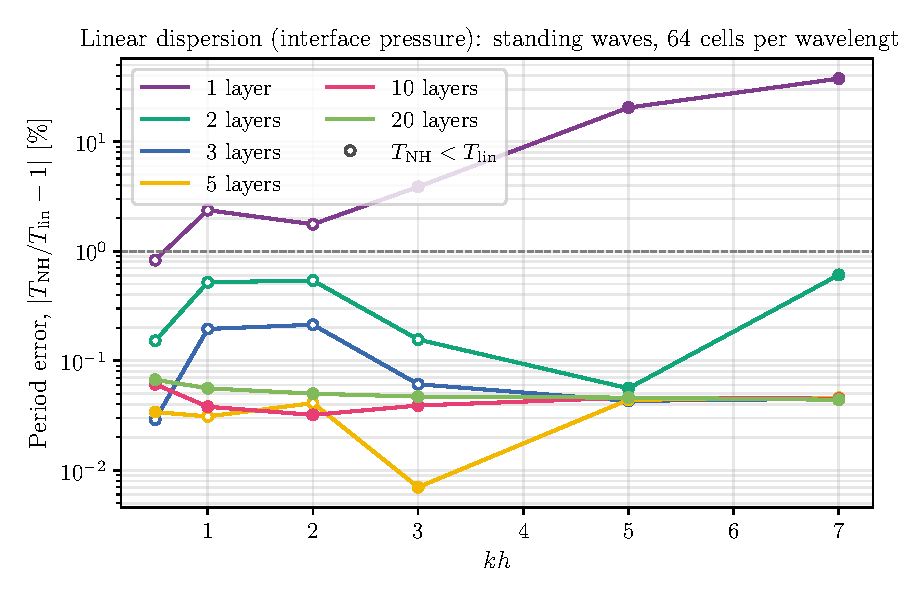
\includegraphics[width=0.85\textwidth]{dispersion_vs_layers.pdf}
\caption{Period error of standing waves against $kh$ for 1--20 uniform layers
(interface pressure). Open symbols: periods shorter than linear theory.}
\label{fig:dispersion}
\end{figure}

Refining the layers towards the surface no longer helps
(Fig.~\ref{fig:grading}). With three layers, a top layer a quarter of the
bottom one moves the error at $kh = 1$--2 from $-0.2\%$ to $-0.45\%$, and at
$kh=5$ it stays at $+0.05\%$. In the cell layout the same grading cut the error
at $kh=5$ from 5.8\% to 2.1\% with five layers.

\begin{figure}[ht]
\centering
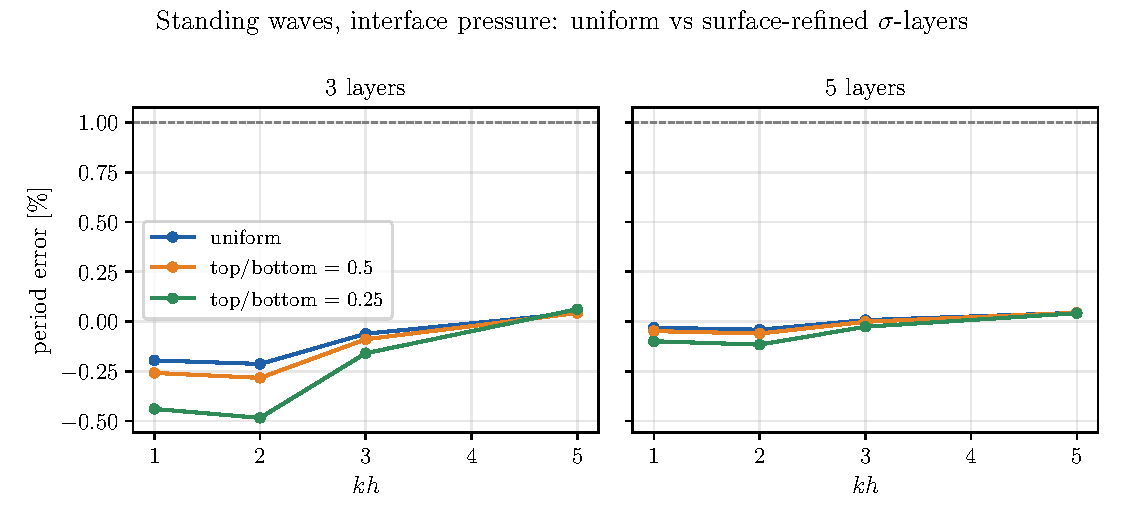
\includegraphics[width=\textwidth]{layer_grading.pdf}
\caption{Period error with uniform and surface-refined layers (interface
pressure).}
\label{fig:grading}
\end{figure}

Against NHWAVE, on the same basins and with the same analysis
(Fig.~\ref{fig:dispmodels}), NHWAVE keeps the period error within 0.8\% with
two layers and 0.45\% with three; \NHFOAM\ within 0.61\% and 0.21\%. With
10--20 layers both converge, NHWAVE to $-0.17\%$ and \NHFOAM\ to $+0.05\%$.
NHWAVE damps more: after 4.5 periods it has lost 0.6--12\% of the amplitude
with three layers and 0.6--3.5\% with ten, \NHFOAM\ 0.04--1.3\% and
0.04--0.7\%.

\begin{figure}[ht]
\centering
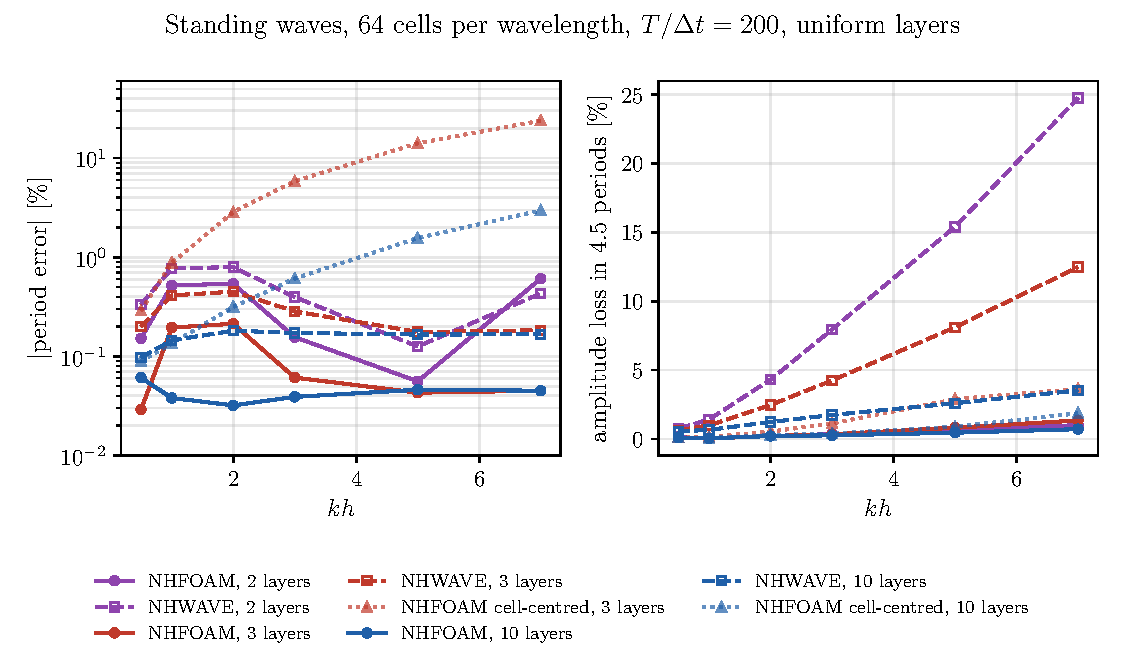
\includegraphics[width=\textwidth]{dispersion_models.pdf}
\caption{Standing waves: period error and amplitude loss of \NHFOAM\ (interface
and cell-centred pressure) and NHWAVE for 2, 3 and 10 uniform layers.}
\label{fig:dispmodels}
\end{figure}

\FloatBarrier
\subsection{Convection and the decay of progressive waves}
\label{sec:convtests}

Waves of $H=4.1$ cm and $T=1.01$ s in 0.4 m of water ($kh = 1.69$, 10 layers,
$\Delta x = 2$ cm) lose 6.1\% of their height over 12 m (8 wavelengths) with
\code{linearUpwind}, 4.7\% with \code{LUST}, 4.4\% with \code{limitedLinearV}
and 3.9\% with central differencing (Fig.~\ref{fig:flume}). With the
cell-centred pressure the same runs lost 12\%, 6.2\%, 3.3\% and 1.7\%. Waves of
$H = 0.4$ cm lose 0.7\% over 10 m with \code{linearUpwind}, so the damping grows
with steepness. The waves leave the wave-making zone about 4\% higher than the
linear target, a nonlinear effect of generating them with linear theory. The
phase speed of the small waves is 0.24\% below linear theory (10 layers,
$T/\Delta t = 100$), of which about 0.13\% is the BDF2 time step. These runs
predate the flux extrapolation of Section~\ref{sec:time}.

\begin{figure}[ht]
\centering
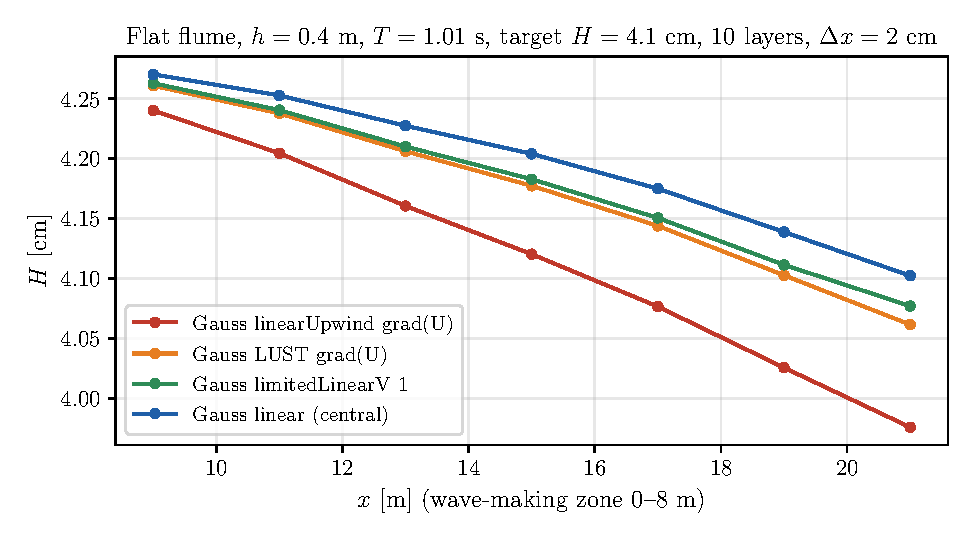
\includegraphics[width=0.85\textwidth]{flume_convection.pdf}
\caption{Wave height along a flat flume for four convection schemes (interface
pressure).}
\label{fig:flume}
\end{figure}

\FloatBarrier
\subsection{Submerged bar}
\label{sec:bar10}

Periodic waves over the submerged bar of \citet{beji1993}, in the version of
\citet{luth1994} with its cases A ($H = 2$ cm, $T = 2.02$ s) and C
($H=4.1$ cm, $T=1.01$ s), test shoaling and the release of free higher
harmonics behind the bar. All three models use $\Delta x = 2$ cm and 10 uniform
layers; \NHFOAM\ uses $\Delta t = 5$ ms. One time shift, fitted at $x=22$ m, is
applied to all gauges of a run, and $\Delta H$ is the error of the wave height
(max $-$ min over the lab record). All runs are compared over the last 4 s
before $t=50$ s (Figs.~\ref{fig:barA} and \ref{fig:barC},
Table~\ref{tab:bar10}).

\begin{table}[ht]
\centering
\caption{Submerged bar, 10 layers: rms error over the 10 gauges and mean
$|\Delta H|/H$, window ending at $t = 50$ s.}
\label{tab:bar10}
\small
\begin{tabular}{lcccc}
\toprule
 & \NHFOAM & \NHFOAM, cell layout & NHWAVE & REEF3D::NHFLOW \\
\midrule
case A, rms        & 0.17 cm & 0.21 cm & 0.29 cm & 0.24 cm \\
case A, $|\Delta H|/H$ & 5.1\% & 6.6\% & 4.7\% & 6.3\% \\
case C, rms        & 0.65 cm & 0.59 cm & 1.02 cm & 0.92 cm \\
case C, $|\Delta H|/H$ & 4.9\% & 4.7\% & 6.1\% & 5.1\% \\
\bottomrule
\end{tabular}
\end{table}

\begin{figure}[p]
\centering
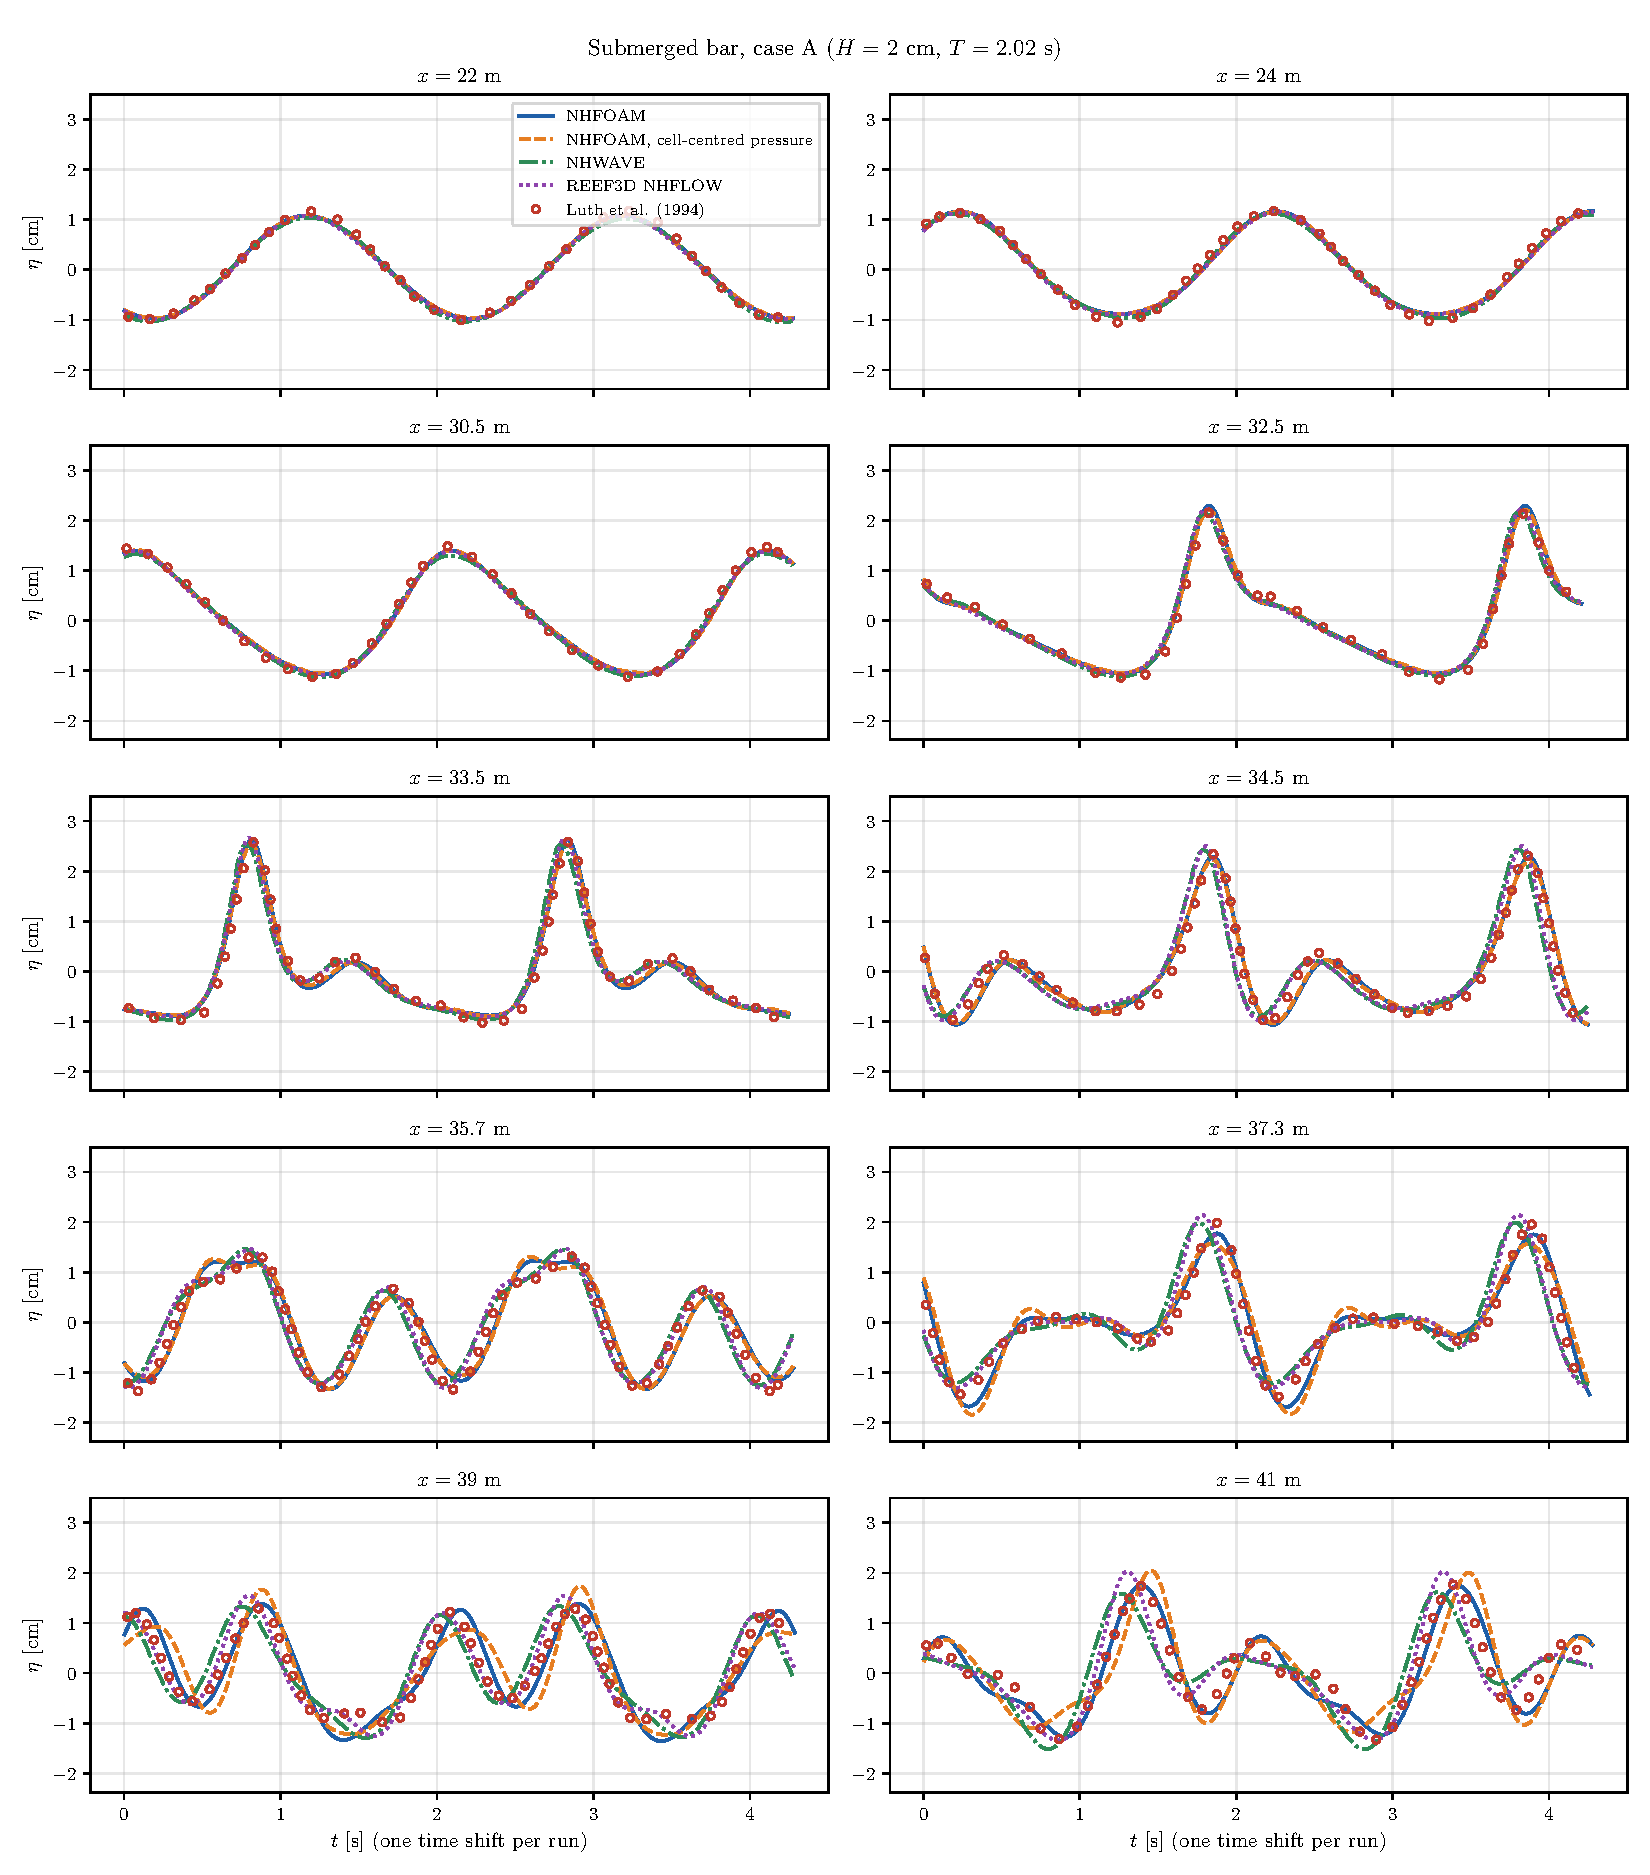
\includegraphics[width=0.9\textwidth]{bar_models_A.pdf}
\caption{Submerged bar, case A, 10 layers: \NHFOAM\ (interface and cell-centred
pressure), NHWAVE and REEF3D::NHFLOW against \citet{luth1994}.}
\label{fig:barA}
\end{figure}

\begin{figure}[p]
\centering
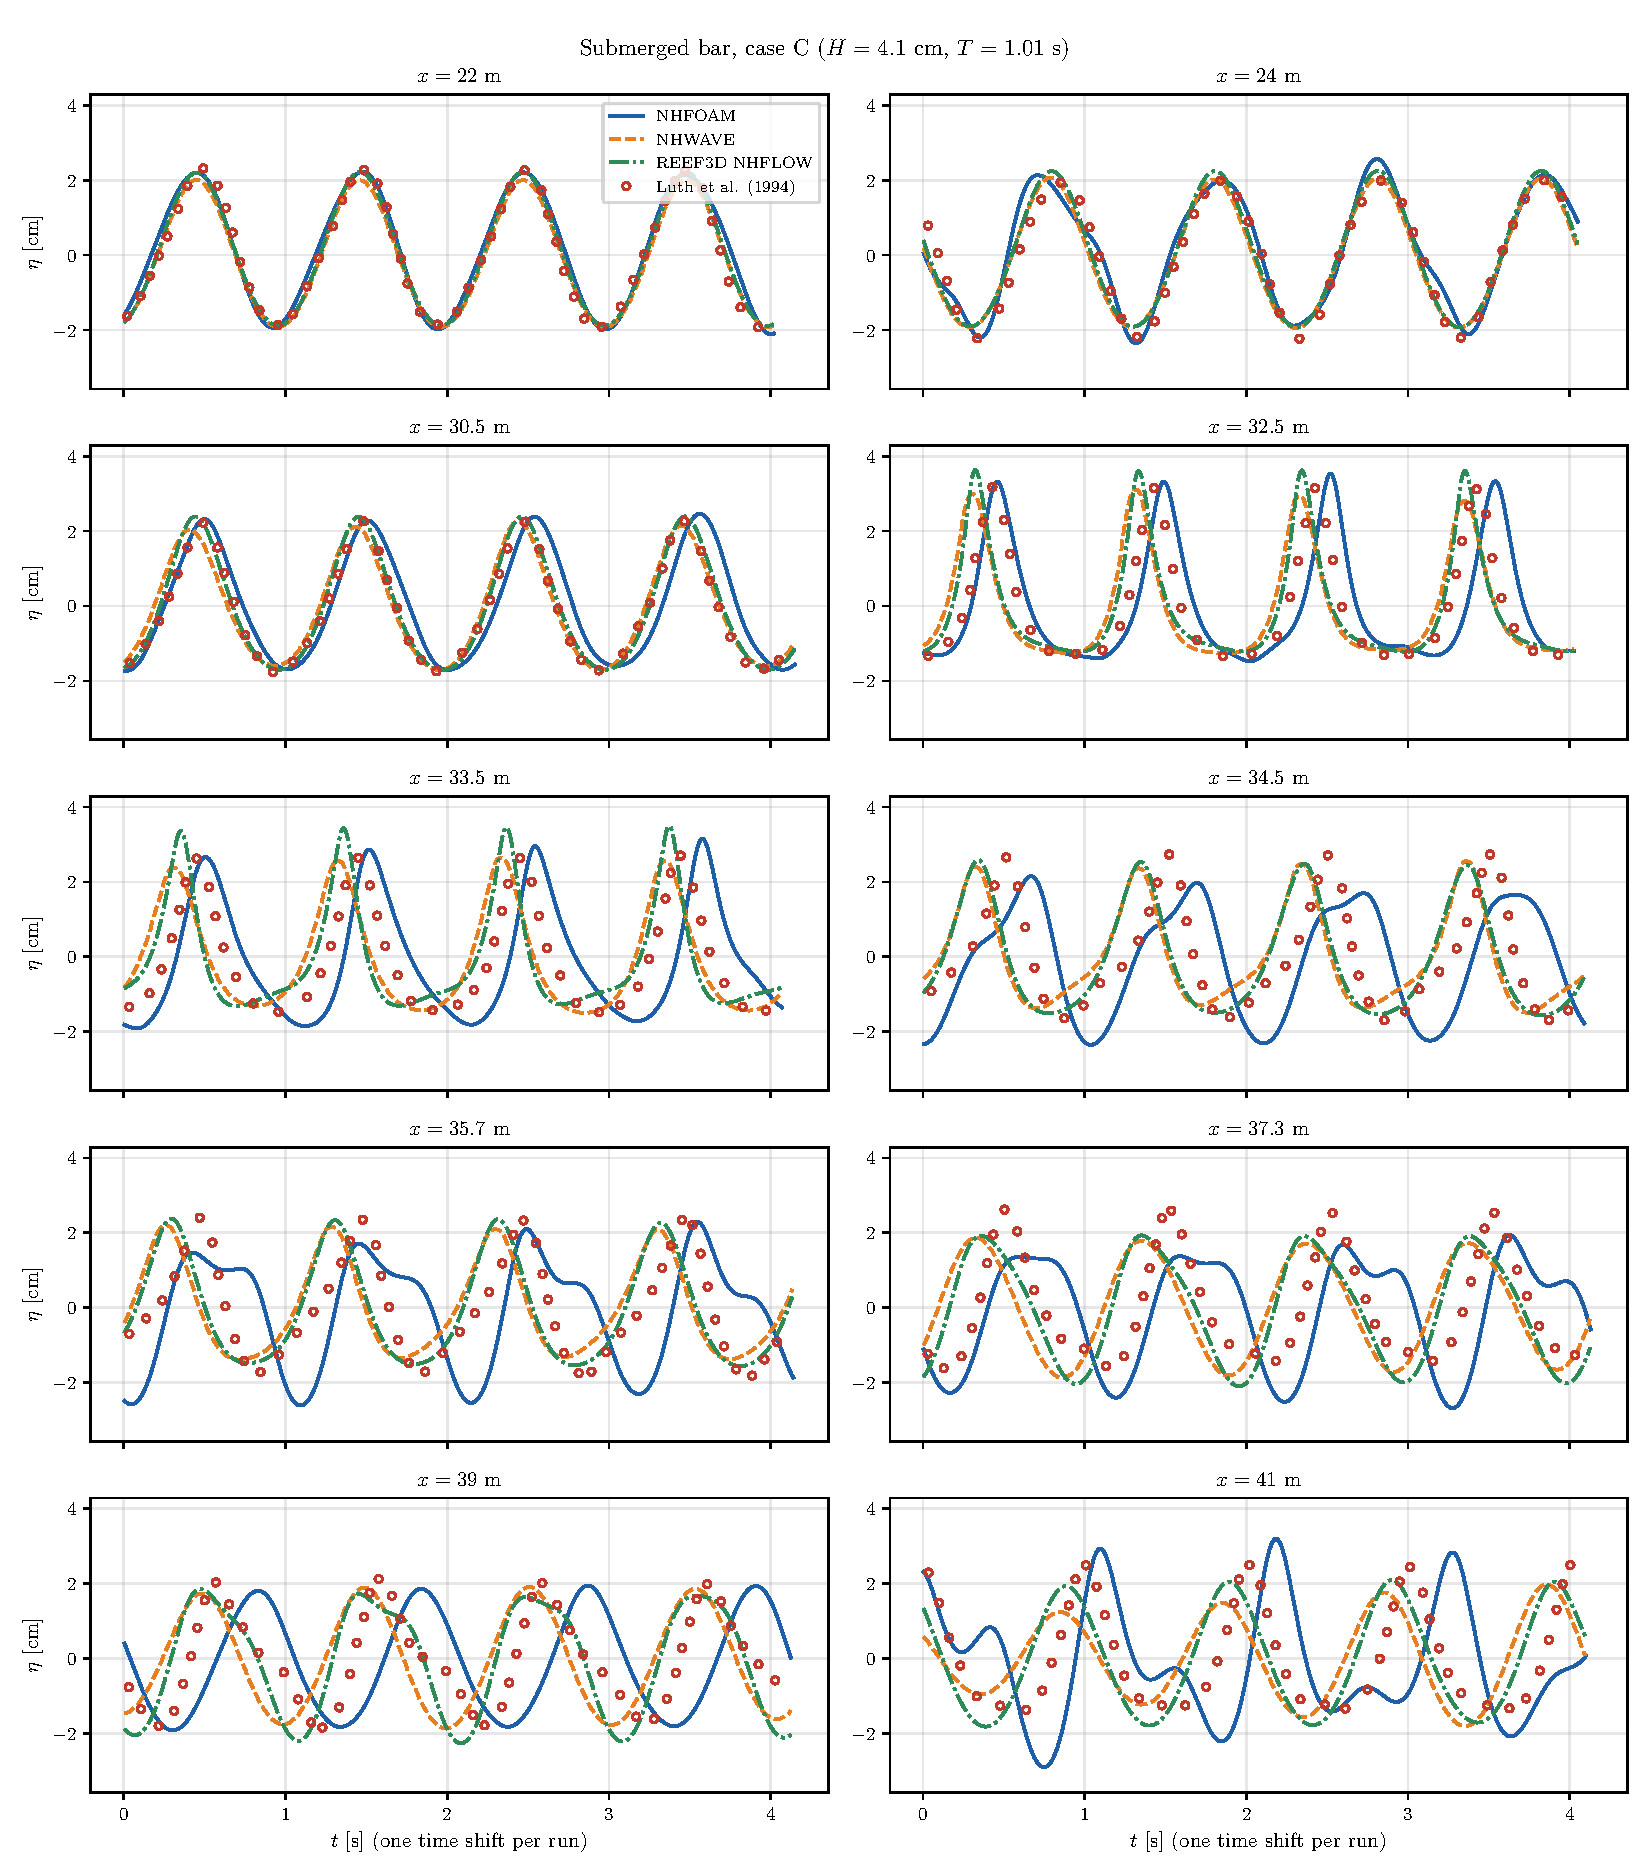
\includegraphics[width=0.92\textwidth]{bar_models_C.pdf}
\caption{As Fig.~\ref{fig:barA}, case C.}
\label{fig:barC}
\end{figure}

In front of the bar ($x\le 30.5$ m) all models are within 0.06--0.42 cm rms of
the measurements. On and behind the bar, \NHFOAM\ has the smallest errors at
every gauge in case C (0.46--0.90 cm, against 1.0--1.5 cm for the other two)
and at 6 of the 7 gauges in case A. In case C the difference is mostly phase:
NHWAVE and REEF3D::NHFLOW are 0.1--0.18 s early over the bar crest, and
\NHFOAM\ up to 0.1 s late.

\paragraph{Long waves of the flume.} The phase over the bar changes with the
time at which it is measured, in all three models. Between $t=45$ and 65 s, the
first harmonic at $x = 35.7$ m moves relative to $x=22$ m by 0.21 s in \NHFOAM,
0.08 s in NHWAVE and $-0.07$ s in REEF3D::NHFLOW. These changes come with mean
water levels that vary by a few millimetres along the flume ($\pm2$ mm in
\NHFOAM, $\pm1$ mm in the other two): long waves of the closed flume, released
when the wave train starts and when it crosses the bar, which the zones absorb
only partly. Over the 0.1 m deep crest the current of such a wave shifts the
waves by tenths of a second, so the rms error depends on the window
(Table~\ref{tab:barwindow}), and so does the ranking. The drift was later
traced to the missing return current of the wave-making zone; with it, the
runs are steady (Section~\ref{sec:bar-bc}).

\begin{table}[ht]
\centering
\caption{Case C, 10 layers: rms error over the 10 gauges for windows ending at
different times.}
\label{tab:barwindow}
\small
\begin{tabular}{lcccc}
\toprule
window ending at & \NHFOAM & \NHFOAM, cell layout & NHWAVE & REEF3D::NHFLOW \\
\midrule
45 s & 0.49 cm & 0.47 cm & 1.08 cm & 0.93 cm \\
50 s & 0.65 cm & 0.59 cm & 1.02 cm & 0.92 cm \\
55 s & 0.94 cm & 0.77 cm & 0.97 cm & 0.92 cm \\
60 s & 1.18 cm & 1.04 cm & 0.89 cm & 0.98 cm \\
65 s & 1.39 cm & 1.19 cm & 0.77 cm & 1.10 cm \\
\bottomrule
\end{tabular}
\end{table}

Two numerical settings matter as much as the model (cell layout, 50 s
windows). With $\Delta t = 10$ ms instead of 5 ms the rms error was 65\% higher
in case A and 150\% higher in case C: the free third harmonic behind the bar
($T/3 = 0.34$ s in case C) then gets only 34 steps per period. And central
differencing failed after 62 s (case A) and 53 s (case C), while
\code{limitedLinearV} runs to the end.

\FloatBarrier
\subsection{Seabed motion}
\label{sec:seabed}

\paragraph{Bottom uplift.} A block of half-width $b=0.305$ m rises by
$\zeta_0 = 0.5$ mm in $h=5$ cm of water with the exponential history
($t_c = 0.1$ s), as in \citet{hammack1973}. With 5 layers and $\Delta x = 5$ mm the
peaks at $x/b = 0$--20 are within 1.5\% of linear potential theory, and the
dispersive tail follows it (Fig.~\ref{fig:uplift}). The two pressure layouts
differ by less than 2\% of $\zeta_0$ at any gauge.

\begin{figure}[ht]
\centering
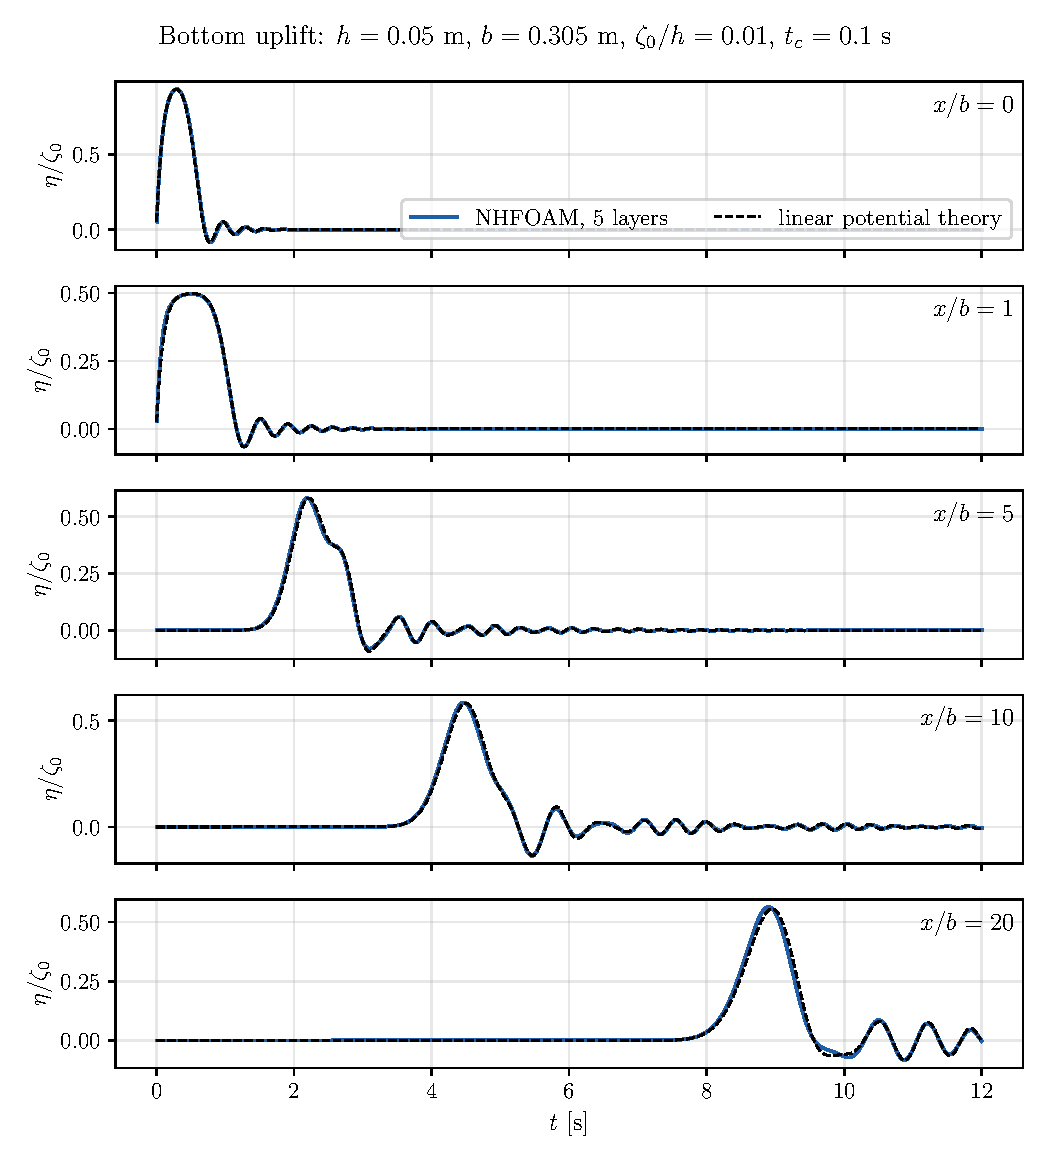
\includegraphics[width=0.8\textwidth]{bottom_uplift.pdf}
\caption{Bottom uplift: gauges against linear potential theory.}
\label{fig:uplift}
\end{figure}

\paragraph{3D rigid landslide.} NTHMP benchmark 2 \citep{enet2007}, $d = 61$ mm:
half tank with a symmetry wall on the axis. \NHFOAM: $\Delta x=\Delta y=2.5$ cm,
5 uniform layers (141\,000 cells), the domain starting 0.2 m from the shoreline
(no wetting and drying). In deep water the layers are up to 12 times thicker
than $\Delta x$, so the interface matrix needs about 180 PCG iterations per solve,
and the run takes 51 min on one core for 4 s. NHWAVE uses its own benchmark
set-up (\code{examples/landslide\_benchmarks/BM2\_enet\_grilli}: $\Delta x = 2$ cm,
3 layers, full beach), with the gauges moved to the published positions. No
time shift is applied (Fig.~\ref{fig:landslide}, Table~\ref{tab:landslide}).

\begin{table}[ht]
\centering
\caption{Landslide, $d=61$ mm: first trough and first crest [mm].}
\label{tab:landslide}
\small
\setlength{\tabcolsep}{4pt}
\begin{tabular}{lcccccccc}
\toprule
 & \multicolumn{4}{c}{first trough} & \multicolumn{4}{c}{first crest} \\
\cmidrule(lr){2-5}\cmidrule(lr){6-9}
gauge $(x,y)$ [m] & lab & \NHFOAM & cell & NHWAVE & lab & \NHFOAM & cell & NHWAVE \\
\midrule
g2 (1.469, 0.35) & $-13.7$ & $-15.3$ & $-14.9$ & $-14.9$ & 15.0 & 16.7 & 15.2 & 16.3 \\
g3 (1.929, 0)    & $-17.0$ & $-17.7$ & $-18.0$ & $-17.1$ & 22.2 & 23.9 & 22.5 & 20.5 \\
g4 (1.919, 0.5)  & $-9.4$  & $-10.2$ & $-9.5$  & $-9.6$  & 11.0 & 13.0 & 11.6 & 12.3 \\
\bottomrule
\end{tabular}
\end{table}

\begin{figure}[ht]
\centering
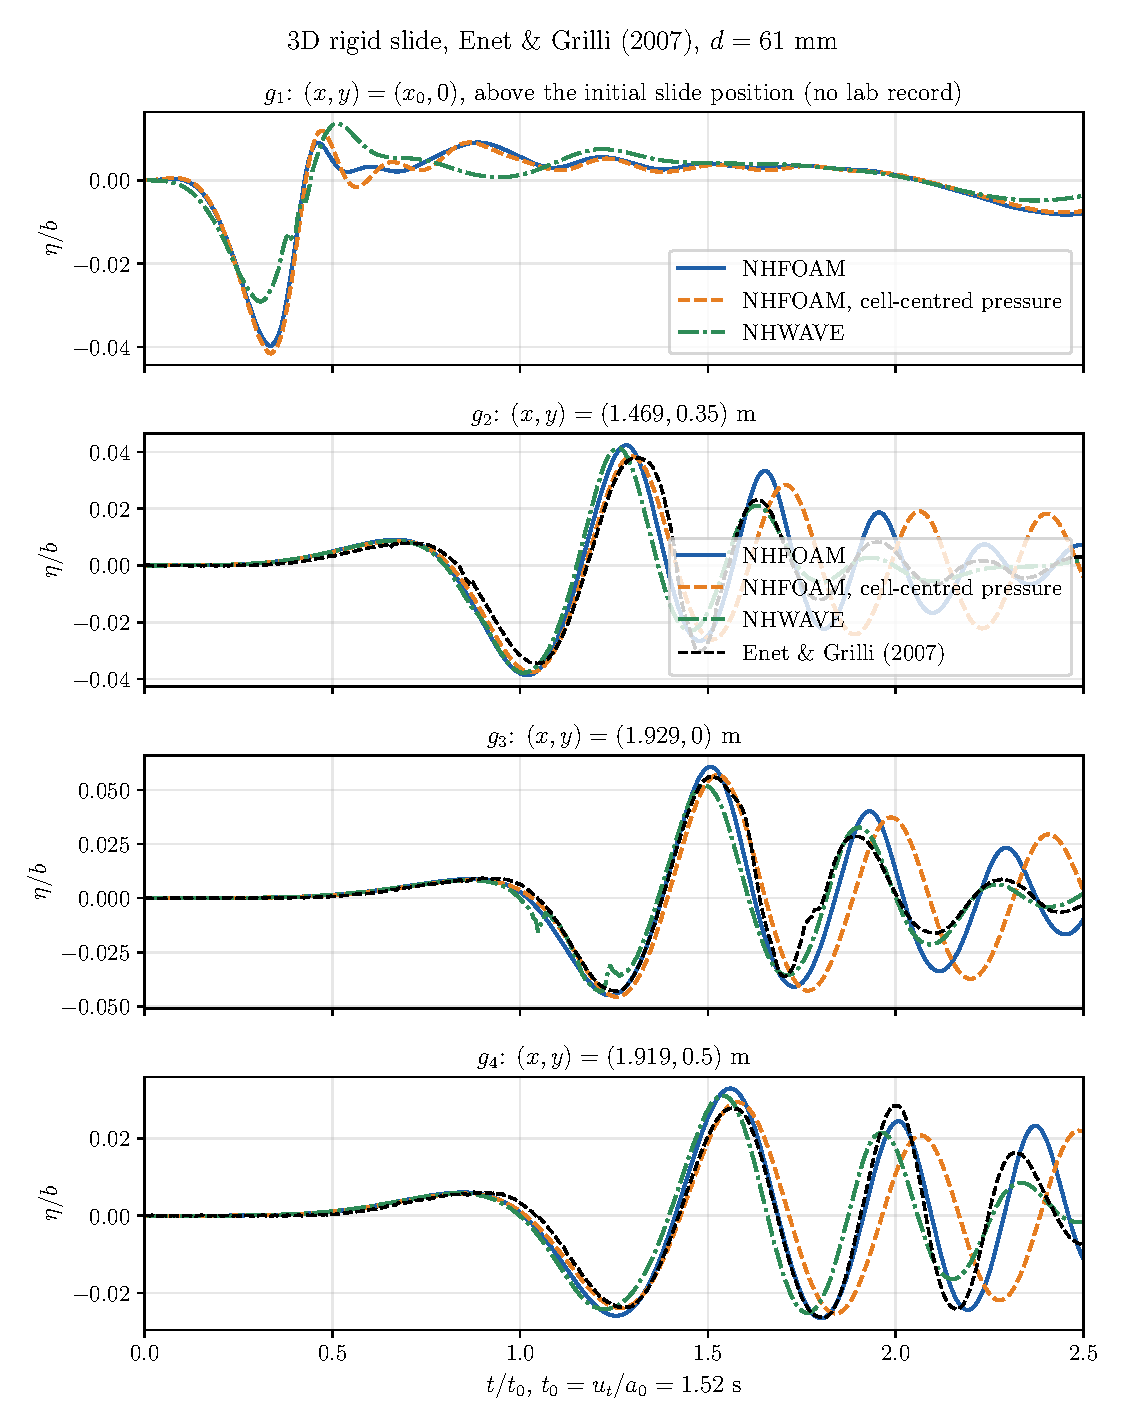
\includegraphics[width=0.85\textwidth]{landslide_models.pdf}
\caption{3D rigid landslide \citep{enet2007}, $d=61$ mm: \NHFOAM\ (interface and
cell-centred pressure) and NHWAVE against the measurements.}
\label{fig:landslide}
\end{figure}

All runs get the leading trough within 12\%. The leading crest is 8--18\% high
with the interface pressure, 1--5\% with the cell-centred pressure, and
between $-7\%$ and $+12\%$ for NHWAVE. \NHFOAM\ has the leading waves on time,
NHWAVE about $0.05\,t_0$ early. The trailing waves ($kh = 3$--5) now follow the
measured phase, as NHWAVE's do; with the cell-centred pressure they fell
further behind with every wave. Their amplitude is still too large: the third
and fourth crests are up to 2--3 times the measured ones, while NHWAVE follows
the measured decay. The wall that replaces \NHFOAM's beach is not the cause
(Section~\ref{sec:ma-landslide}).

\FloatBarrier
\subsection{Breaking}
\label{sec:breaking}

Spilling breakers of \citet{hansen1979}, test 061071: $T = 1.67$ s, $H = 6.9$ cm
at the toe of a 1:34.26 slope from $h=0.36$ m. 10 layers, $\Delta x = 2$ cm,
$\Delta t = 10$ ms, HFA with $\alpha = 0.6$ and $\beta=0.3$, \code{limitedLinearV}.
The slope is cut at $x = 11$ m ($h = 3.9$ cm) and continues as a 3 m shelf with
a velocity-only sponge. The run covers 40 periods, and the statistics use the
last 10 (Fig.~\ref{fig:hs}, Table~\ref{tab:hs}).

\begin{table}[ht]
\centering
\caption{Spilling breakers: wave height (mean of max $-$ min per period).}
\label{tab:hs}
\small
\begin{tabular}{llll}
\toprule
 & lab & \NHFOAM\ (interface) & \NHFOAM\ (cell) \\
\midrule
near the toe, $x<1$ m & 6.9--7.0 cm & $-1\%$ to $+9\%$ & $+8\%$ to $+17\%$ \\
shoaling, $x = 2$--7 m & 7.0--8.4 cm & $-4\%$ to $+20\%$ & $-2\%$ to $+9\%$ \\
largest & 10.4 cm at 8.2 m & 10.9 cm at 8.1 m & 10.6 cm at 9.0 m \\
surf zone, $x = 8.3$--11 m & 10.0 $\to$ 3.5 cm & $+3\%$ to $+99\%$ & $-12\%$ to $+47\%$ \\
rms before / after $x=8.3$ m & & 0.55 / 2.98 cm & 0.56 / 1.79 cm \\
rms over all lab points & & 1.55 cm & 1.01 cm \\
\bottomrule
\end{tabular}
\end{table}

\begin{figure}[ht]
\centering
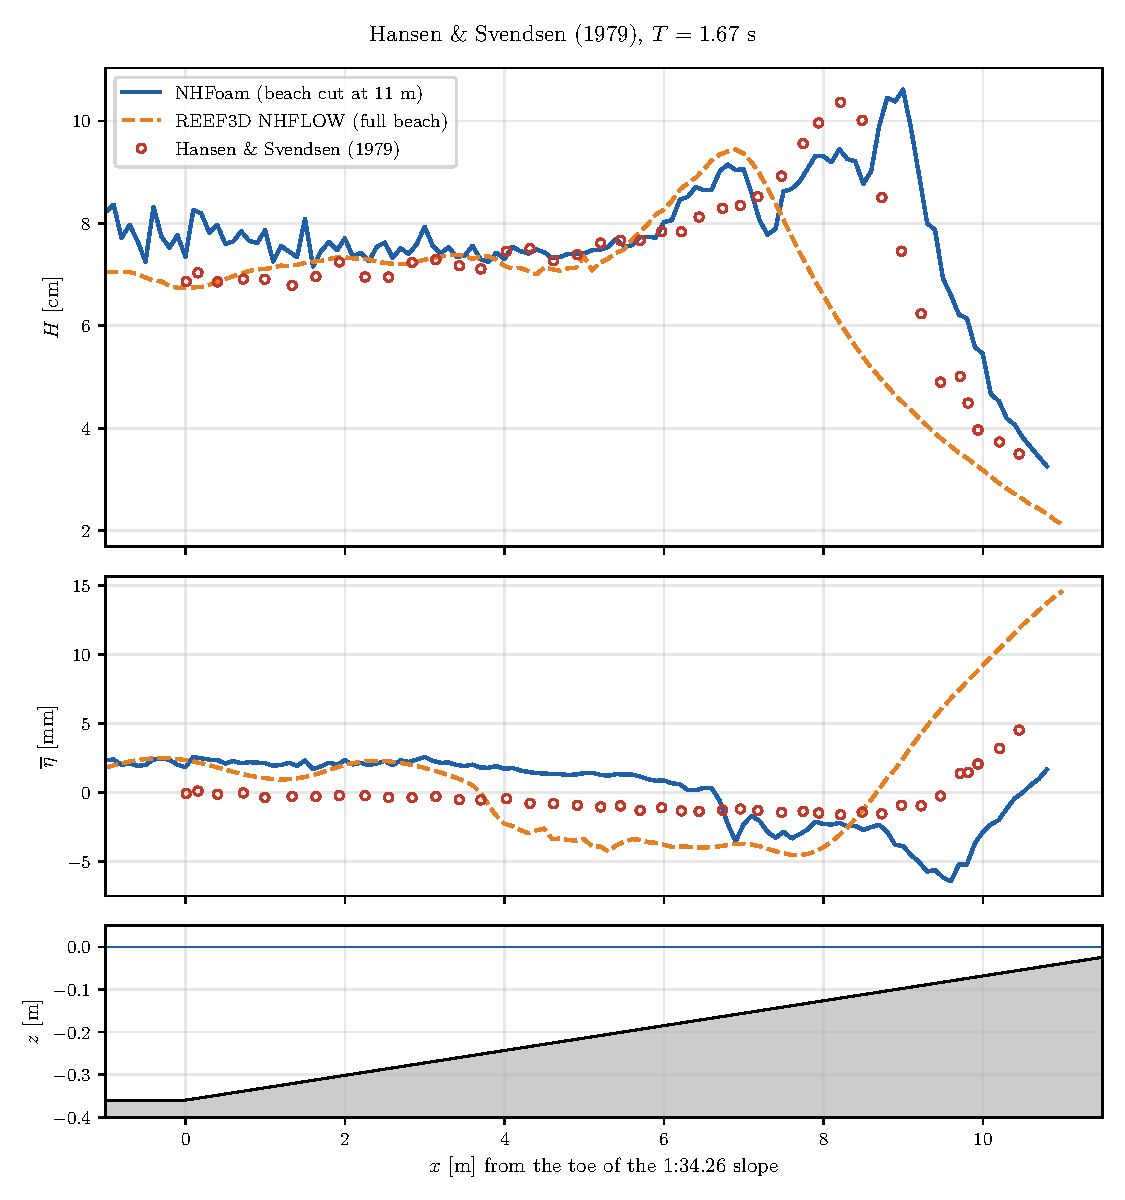
\includegraphics[width=0.85\textwidth]{hansen_svendsen_models.pdf}
\caption{Spilling breakers \citep{hansen1979}: wave height and mean water level.
REEF3D::NHFLOW has the full beach; \NHFOAM\ ends in a shelf with a
velocity-only sponge.}
\label{fig:hs}
\end{figure}

With the interface pressure the incident waves are within a few percent of the
lab at the toe, and the waves break where they did in the flume: the largest
height is 5\% high and 0.1 m from the measured position (the cell layout broke
0.8 m too far inshore). Inside the surf zone, however, the bores lose too
little energy; they keep a sawtooth shape of 7--8 cm down to $x = 10$ m, where
the lab heights have halved. The breaking switch flags about 7 columns at a
time in both layouts, so the onset is right and the dissipation of the
hydrostatic bores is what falls short. REEF3D::NHFLOW, with the full beach and
its own breaking algorithm, breaks too early (largest $H$ 9.4 cm at $x=6.9$ m,
rms 1.5 cm). Without a beach, \NHFOAM\ does not reproduce the mean water level.
NHWAVE is not included: our run of this case (10 layers, $k$--$\epsilon$, full
beach) stopped after 4 s without an error message.

The bore fronts are where the lagged terms of the interface matrix matter
most. With only $A^2$ in the implicit vertical coefficient of
\eqref{eq:midflux}, the pressure correctors diverged under the first steep
bores after 22 s, with a fixed or an adaptive time step alike; the
over-relaxed split fixed it. Bores also need a TVD convection scheme
everywhere: with central differencing away from the breaking columns,
grid-scale oscillations grow behind the bores.
